\documentclass[a4paper]{article}

%% Language and font encodings
\usepackage[english]{babel}
\usepackage[utf8x]{inputenc}
\usepackage[T1]{fontenc}

%% Sets page size and margins
\usepackage[a4paper,top=3cm,bottom=2cm,left=3cm,right=3cm,marginparwidth=1.75cm]{geometry}

%% Useful packages
\usepackage{amsmath}
\usepackage{graphicx}
%\usepackage{url}
\usepackage{hyperref}
\usepackage[colorinlistoftodos]{todonotes}
\usepackage{hyperref}
\usepackage{pgfplots}
\pgfplotsset{compat=1.9}

\usepackage{tikz}
\usetikzlibrary{decorations.pathmorphing,patterns}
\usetikzlibrary{external}
\tikzexternalize

\title{What is a photon?}
\author{Dan Piponi}

\begin{document}
\maketitle

\begin{abstract}
Popular science writing about quantum mechanics leaves many people full of questions about the status of photons.
I want to answer some of these without using any tricky mathematics.

One of the challenges is that photons are very different to ordinary everyday objects like billiard balls.
This is partly because photons are described by quantum mechanics whereas billiard balls are better modelled with classical Newtonian mechanics.
Quantum mechanics defies many of our intuitions.
But it's also because the word {\em photon} plays by different linguistic rules to {\em billiard ball}.
I hope to explain why in a way.

One of my goals is to avoid saying anything original.
I'm largely going remove the mathematics from material I first learnt from three or so courses I took at Cambridge University many years ago: Quantum Mechanics, Solid State Physics and Quantum Field Theory.
I also learnt about some of this from David Miller at Stanford University who talked a little about what properties it is meaningful to apply to a photon.
(I hope I haven't misrepresented him too badly.)
\end{abstract}

\section{The simple harmonic oscillator}

Here's a mass hanging on a spring:

\begin{center}
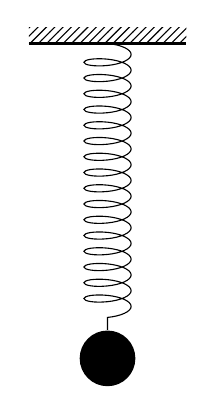
\begin{tikzpicture}
\node[circle,fill=black,inner sep=2.5mm] (a) at (0,0) {};
%\node[circle,fill=blue,inner sep=2.5mm] (b) at (2,2) {};
\draw[decoration={aspect=0.3, segment length=2mm, amplitude=3mm,coil},decorate] (0,4) -- (a); 
%\draw[decoration={aspect=0.3, segment length=1.5mm, amplitude=3mm,coil},decorate] (2,5) -- (b); 
\fill [pattern = north east lines] (-1,4) rectangle (1,4.2);
\draw[thick] (-1,4) -- (1,4);
\end{tikzpicture}
\end{center}

Suppose it's initially sitting in equilibrium so that the net force acting on it is zero.
Now we lift the mass a small distance and let it go.
Because we lifted it, we shortened the spring, reducing its tension.
This means the force due to gravity is now more than the spring tension and the mass falls.
Eventually it falls below the equilibrium point, increasing the tension in the spring so there is a net force pulling it back up again.
To a good approximation, the force restoring the mass to its equilibrium point is proportional to how far it has been displaced.
When this happens we end up with oscillating motion where the mass bounces up and down.
Here's what a graph of its displacement looks like over time:

\begin{center}
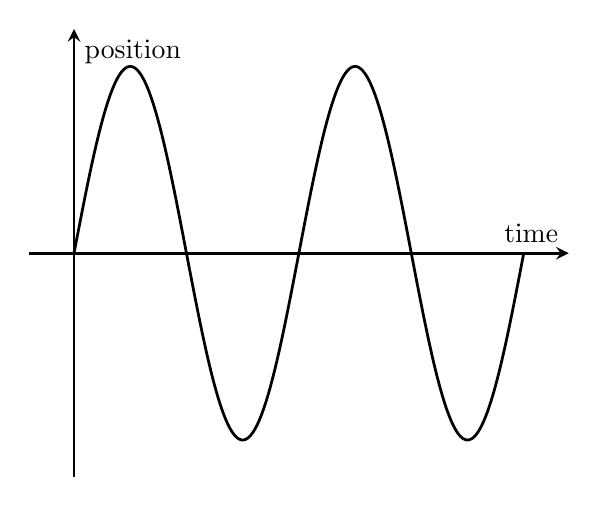
\begin{tikzpicture}
  \begin{axis}[
    axis lines = middle,
    xlabel = time,
    ylabel = position,
    enlargelimits,
    clip=false,
    ticks=none,
    line width = 1pt,
    xticklabels={,,},
    yticklabels={,,}
    ]
    \addplot[domain=0:720,samples=200,black,line width=1pt] {sin(x)};
%    \draw[dotted,blue!40] (axis cs: 0.5*pi,1.1) -- (axis cs: 0.5*pi,0);
%    \draw[dotted,red!40] (axis cs: 0.5*pi+2,1.1) -- (axis cs: 0.5*pi+2,0);
  \end{axis}
\end{tikzpicture}
\end{center}
It's actually a sine wave but that detail doesn't matter for us right now.

An oscillator where the restoring force is proportional to the displacement from the equilibrium point is called a {\em simple harmonic oscillator}\footnote{See \url{https://en.m.wikipedia.org/wiki/Simple_harmonic_motion}} and its oscillation is always described by a sine wave.

Note that I'm ignoring friction here. This is a reasonable approximation for many physical systems.

Masses on springs aren't all that important in themselves.
But simple harmonic oscillators are very common.
Another standard example is the pendulum swinging under the influence of gravity:

\begin{center}
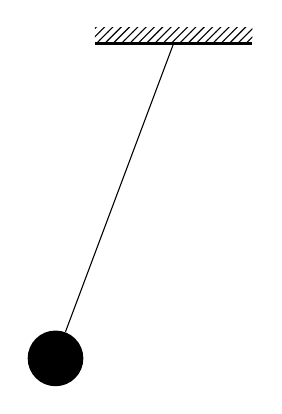
\begin{tikzpicture}
\node[circle,fill=black,inner sep=2.5mm] (a) at (-1.5,0) {};
%\node[circle,fill=blue,inner sep=2.5mm] (b) at (2,2) {};
\draw[decoration={aspect=0.3, segment length=2mm, amplitude=3mm},decorate] (0,4) -- (a); 
%\draw[decoration={aspect=0.3, segment length=1.5mm, amplitude=3mm,coil},decorate] (2,5) -- (b); 
\fill [pattern = north east lines] (-1,4) rectangle (1,4.2);
\draw[thick] (-1,4) -- (1,4);
\end{tikzpicture}
\end{center}

At a more fundamental level, an example might be an atom in a crystal being held in place by electrostatic forces from its neighbouring atoms.

If you have one of these systems, then in principle you can set it in motion with as little energy as you like.
Pull a mass on a spring down a little bit and it will bounce back up, oscillating a certain amount.
Pull the mass down half the amount and it'll bounce with oscillations half the size.
In principle we could keep repeating this experiment, each time starting with the mass displaced half the amount we tried previously.
In other words, a simple harmonic oscillator can have any energy we like.
The {\em spectrum} of possible energies of one of these oscillators is continuous.
(Note that the word {\em spectrum} here is merely physicist-speak for a set of possible values.)
If we can set one in motion with 1 unit of energy then we can also set it oscillating with 0.5 units, or 0.01 units, or 0.000123 units of energy.

\section{Quantum mechanics}

Everything I've said above is assuming that classical Newtonian mechanics is valid.
But we know that for very small systems, around the size of a few atoms or smaller, we need to use quantum mechanics.
This is an enormous topic but I'm only going to extract one basic fact.
According to quantum mechanics, a simple harmonic oscillator isn't free to oscillate with any energy you like.
The possible energy levels, the spectrum of the system, is discrete.
There is a lowest energy level, and then all of the energy levels above that are equally spaced like so, going up forever:

\begin{center}
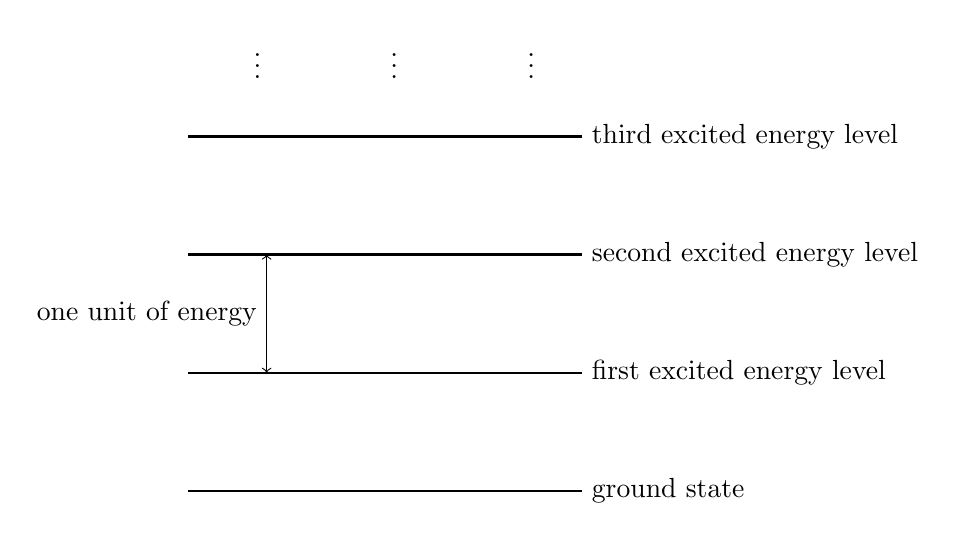
\begin{tikzpicture}
\coordinate (dash) at (0,0);
\coordinate[below=1cm of dash] (psii);
\coordinate[below=1.5cm of psii] (psif);
\coordinate[below=1.5cm of psif] (psig);
\coordinate[below=1.5cm of psig] (psih);

\draw[thick] (dash) node[right]{\qquad $\vdots$ \hskip 0.6in $\vdots$ \hskip 0.6in $\vdots$};
%\draw[thick] (dash)--++(0:5cm) node[right]{$\vdots$};
\draw[thick] (psii)--++(0:5cm) node[right]{third excited energy level};
\draw[thick] (psif)--++(0:5cm) node[right]{second excited energy level};;
\draw[thick] (psig)--++(0:5cm) node[right]{first excited energy level};;
\draw[thick] (psih)--++(0:5cm) node[right]{ground state};;

\draw[<->] ([xshift=1cm]psig) -- ([xshift=1cm]psif) node[left, midway] (hwi) {one unit of energy};
%\draw[<-] ([xshift=3cm]psif) -- ([xshift=3cm]dash) coordinate(aux);
%\path (aux|-hwi) node[right] {{$\omega_S$}};
\end{tikzpicture}
\end{center}

We usually call the lowest energy level the {\em ground state}\footnote{See \url{https://en.m.wikipedia.org/wiki/Vacuum_state}} or {\em vacuum state} and call the higher levels {\em excited} states.

The spacing of the energy levels depends on the {\em stiffness} of the system, which is just a measure of how much the restoring force increases with displacement from equilibrium. Stiffer systems will have a higher frequency of oscillation and a bigger spacing between the energy levels.

(I'm deliberately not saying anything about why we get discrete energy levels in quantum mechanics. I just want to use this one fact so I can get on and talk about photons eventually.)

In practice the difference in energy between one level and the next is tiny. This means that if you're literally fiddling about with a mass on a spring you won't ever feel the discreteness. The amount your hand trembles is many orders of magnitude greater than the effect of this discreteness. Nonetheless, it is extremely important when modeling microscopic systems.

\section{Quantum linguistics}

Here are some English sentences we could say about the kinds of systems I've described so far:

\begin{enumerate}
\item This system is in the ground state.
\item That system is in its first excited state
\item This system is at an energy level higher than that system
\item After allowing these two similar oscillators to interact, the energy level of this oscillator went down and the energy level of that one went up by the same amount.
\end{enumerate}

Now I want to introduce the (count) noun {\em quantum}\footnote{See \url{https://en.m.wikipedia.org/wiki/Quantum}}, with plural {\em quanta}.
The idea here is not that I'm telling you about a new entity.
I want to present this as a new way to talk about things I've already introduced.
So rather than give a definition of {\em quantum} I will instead show how you can rewrite the above sentences using the language of quanta:

\begin{enumerate}
\item There are no quanta in this system
\item That system has one quantum of energy
\item This system has more quanta than that one
\item Some quanta were transferred from this system to that system.
\end{enumerate}

Those sentences make it seem like I'm talking about a new kind of object - the quantum.
But I'm not.
They're just a manner of speaking about energy levels.
I hope I've given you enough examples to get the idea.

Just in case you think it's weird to talk about energy levels in terms of quanta, I'd like to remind you that you already do this all the time with money.
Dollar bills are actual objects that exist in the world.
But money in your bank account isn't.
Somewhere in some database is a representation of how much money you have.
You might say ``I have one hundred dollars in my savings account''
But those dollars certainly don't exist as distinct entities.
It doesn't really make sense to talk about the thirty-seventh dollar in your bank account.
You can transfer dollars from one account to another, and yet what's really happening is that two totals are being adjusted.
We treat these accounts a lot like they're containers holding individual objects called dollars.
Certainly our language is set up like that.
But we know that it's really just the totals that have any kind of representation.
The same goes for quanta.
It's just a manner of speaking about systems that can have different amounts of energy and where the spectrum of energy levels forms a ladder with equally spaced rungs.
Because of your experience with money I probably don't need to give you any more examples.

One more bit of terminology: when the spectrum of energies is discrete it's said to be {\em quantised}.

\section{Coupled systems}

Let's return to classical physics with a slightly more complex system consisting of two masses connected to springs. We ignore gravity now:

\begin{center}
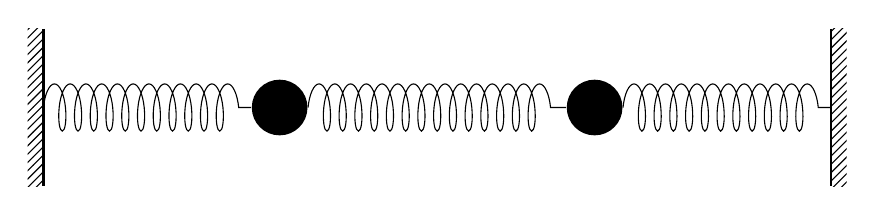
\begin{tikzpicture}
\node[circle,fill=black,inner sep=2.5mm] (a) at (0,0) {};
\node[circle,fill=black,inner sep=2.5mm] (b) at (4,0) {};
\draw[decoration={aspect=0.3, segment length=2mm, amplitude=3mm,coil},decorate] (a) -- (b); 
%\fill [pattern = north west lines] (-4,0) rectangle (4.2,1);

\draw[decoration={aspect=0.3, segment length=2mm, amplitude=3mm,coil},decorate] (-3,0) -- (a); 
\draw[decoration={aspect=0.3, segment length=2mm, amplitude=3mm,coil},decorate] (b) -- (7,0); 

\fill [pattern = north east lines] (-3.2,1) rectangle (-3,-1);
\draw[thick] (-3,1) -- (-3,-1);

\fill [pattern = north east lines] (7.2,1) rectangle (7,-1);
\draw[thick] (7,1) -- (7,-1);

\end{tikzpicture}
\end{center}

We restrict ourselves to just considering back and forth motion constrained along a horizontal line.
This is a coupled system.
If the left mass moves to the right, not only does it experience a restoring force pushing it left, but the mass on the right will experience more of a force pushing it to the left.
We can't treat the masses as independent and so we don't get the simple solution of each mass always oscillating with a sine wave.

For this particular problem though there's a trick to turn it into a pair of harmonic oscillators.
The idea is to consider the pair of masses as a single entity.
We can think of the motion centre of mass of the pair, the midpoint between them, as being one variable that describes this entity.
Let's call its motion the {\em external} motion.
We can also think of the distance between the two masses in the pair as being the system's {\em internal} motion.
(I'm just using {\em internal} and {\em external} as convenient names.
Don't read too much into them.)
It turns out that when you analyse this using classical dynamics the internal motion and the external motion act like independent quantities.
What's more, each one behaves exactly like it's simple harmonic.
So we get one sine wave describing the overall motion of the pair, and another one that describes how the elements of the pair oscillate with respect to each other.

The frequencies of the internal and external motions are typically different.
So you can end up with some quite complicated motions with two different frequencies beating against each other.

When we're able to find ways to split up the motion into independent quantities, each of which is simple harmonic, each kind of motion is said to be a {\em normal mode}\footnote{See \url{https://en.m.wikipedia.org/wiki/Normal_mode}}.

When you have independent normal modes, you can treat them independently in quantum mechanics too.
So what we get is that the spectrum of possible energy levels for this system is, in some sense, two-dimensional.
We can put quanta into the internal oscillation and we can also put quanta into the external oscillation.
Because these modes have different frequencies the quanta for each mode correspond to different amounts of energy.

(And a reminder: when talking about quantum mechanics I'm not talking literally about masses on springs. I'm talking about physical systems that have equations of motion that mean they behave like masses on springs. In this case it might be a pair of particles trapped in a microscopic well with a repulsive force between them.)

\section{Solid state physics}
Now I'm going to jump from just two masses to a large number of them.
For example, the behavior of trillions of atoms in a solid crystal can be approximately modelled by a grid of masses and springs, of which the following diagram is just a tiny piece:

\begin{center}
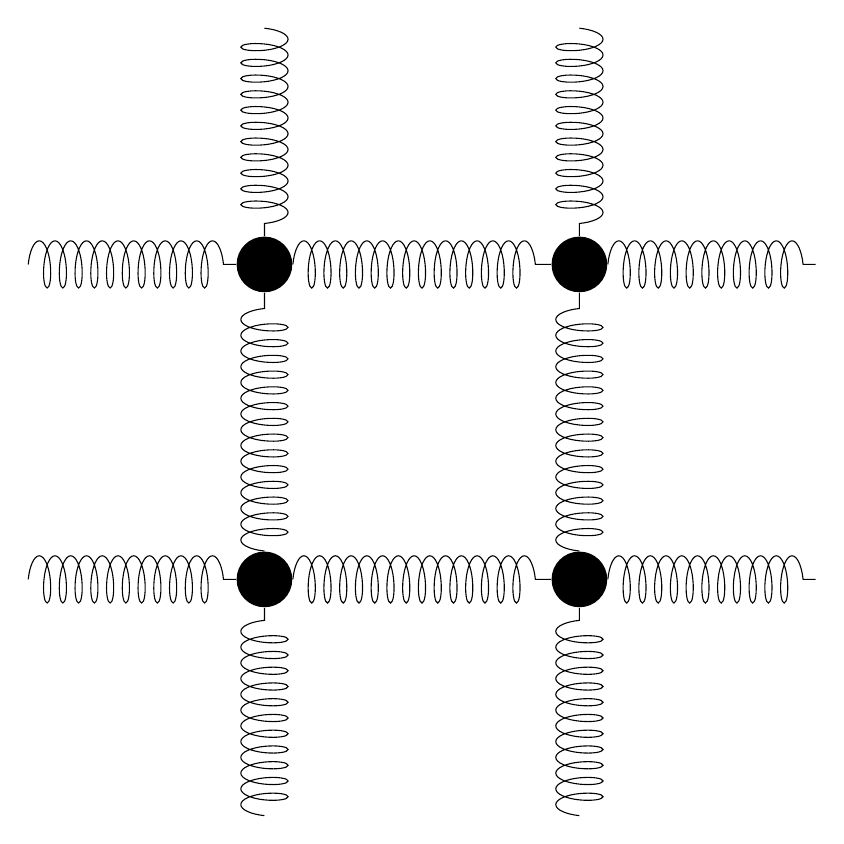
\begin{tikzpicture}
\node[circle,fill=black,inner sep=2.5mm] (a) at (0,0) {};
\node[circle,fill=black,inner sep=2.5mm] (b) at (4,0) {};
\node[circle,fill=black,inner sep=2.5mm] (c) at (0,4) {};
\node[circle,fill=black,inner sep=2.5mm] (d) at (4,4) {};

\draw[decoration={aspect=0.3, segment length=2mm, amplitude=3mm,coil},decorate] (a) -- (b); 
\draw[decoration={aspect=0.3, segment length=2mm, amplitude=3mm,coil},decorate] (c) -- (d); 
\draw[decoration={aspect=0.3, segment length=2mm, amplitude=3mm,coil},decorate] (a) -- (c); 
\draw[decoration={aspect=0.3, segment length=2mm, amplitude=3mm,coil},decorate] (b) -- (d); 
\draw[decoration={aspect=0.3, segment length=2mm, amplitude=3mm,coil},decorate] (-3,0) -- (a); 
\draw[decoration={aspect=0.3, segment length=2mm, amplitude=3mm,coil},decorate] (b) -- (7,0); 
\draw[decoration={aspect=0.3, segment length=2mm, amplitude=3mm,coil},decorate] (-3,4) -- (c); 
\draw[decoration={aspect=0.3, segment length=2mm, amplitude=3mm,coil},decorate] (d) -- (7,4); 
\draw[decoration={aspect=0.3, segment length=2mm, amplitude=3mm,coil},decorate] (0,-3) -- (a); 
\draw[decoration={aspect=0.3, segment length=2mm, amplitude=3mm,coil},decorate] (4,-3) -- (b); 
\draw[decoration={aspect=0.3, segment length=2mm, amplitude=3mm,coil},decorate] (0,7) -- (c); 
\draw[decoration={aspect=0.3, segment length=2mm, amplitude=3mm,coil},decorate] (4,7) -- (d); 

\end{tikzpicture}
\end{center}


A real crystal would be arranged in a 3D lattice but I've drawn 2D here for convenience.

Think of the springs as both pushing apart atoms that get close, and pulling together atoms that move apart.

This is a highly coupled system.
Ultimately every atom in our lattice is connected to every other one, either directly, or indirectly.
Nonetheless, it is still possible to find normal modes.
The normal modes all have the same basic form:
they are all sinusoidal waves of displacement traveling in some direction with some speed and oscillation frequency.
Each of these modes consists of waves that extend through the entire crystal, with fixed spacing between parallel planar wavefronts.
This type of waves is known as a plane wave.
If the system is perfectly harmonic, so the restoring force is precisely proportional to the displacement, then each direction and frequency of wave oscillates its way through the crystal completely independently of any other.
Just as how in the example with two masses any possible oscillation is a combination of internal and external motion, for a crystal lattice any motion is a combination of these plane waves.
(Decomposing any oscillation as a combination of plane waves is known as computing its Fourier transform.\footnote{See \url{https://en.m.wikipedia.org/wiki/Fourier_transform}})

Now we're ready to consider this situation quantum mechanically.
Because each plane wave is a normal mode, we can treat each one as an independent simple harmonic oscillator.
This means that the energy in each plane wave is quantised.
So when we consider a crystal lattice quantum mechanically we find that its states consist of plane waves propagating through it, but where the amount of energy in each wave is given by a discrete spectrum.
So again we can talk about how many quanta there are in each mode.

Linguistically it gets a bit more interesting now.
Each plane wave is associated with a particular direction and speed so it makes sense to talk of these quanta as having a direction and speed.
But note that statements involving quanta are still really just sentences about energy levels.
So, for example, the statement ``the mode of this system with this velocity and frequency is in its first excited state'' is, by definition, exactly the same as ``this system has precisely one quantum with this velocity and frequency''.
In particular, when we write sentences like these we aren't implying that there is some new kind of object, the quantum, that has suddenly attached itself to our crystal.
The quanta are properties of the lattice.
By the way, in the particular case of vibrating atoms in a lattice, the quanta are known by a special name: {\em phonons}\footnote{See \url{https://en.m.wikipedia.org/wiki/Phonon}}.

\section{Quantum field theory and photons}
And now we're ready to move onto photons.

In classical physics, electromagnetism is described by Maxwell's equations.
Maxwell's equations say that a varying magnetic field generates an electric field and a varying electric field generates a magnetic field.
The result is that it is possible for an oscillating electric field to create an oscillating electric field so that an electric field can propagate through space on its own without the help of electric charges or electric currents or any other kind of `generator'.
As these electric fields also produce magnetic fields that propagate with them, the whole thing is called an electromagnetic wave.

Just like displacements in a crystal lattice, an electromagnetic wave also has normal modes.
The normal modes are plane waves traveling at the speed of light in a particular directions with a given frequency.
You have personal experience of this.
Visible light is electromagnetic radiation with a frequency of around 500 THz.
Wifi uses signals at around 5 GHz.
The radio might use signals at around 100 MHz.
When you surf the web wirelessly while listening to the radio, the wifi signals don't interfere with your vision or the radio signal.
(Actually, wifi might interfere with the radio signals, but not because of the 5 GHz signals. It might happen if badly manufactured hardware emits stray signals around the 100 MHz band.)
That's because these waves pass through each other without being coupled to each other in any way.
And at this point you might already be guessing what a {\em photon} is.
For each choice of frequency and direction (and also polarisation, but that's just a detail) the amount of energy that can be in the corresponding mode is quantised.
For the electromagnetic field the quanta are called photons.\footnote{See \url{https://en.m.wikipedia.org/wiki/Photon}}

And that's it!

Electromagnetic waves can be thought of as being made up of different oscillation modes.
Because of quantum mechanics, each mode contains an amount of energy that is quantised to be a whole number multiple of some base amount.
Although the thing that really matters is the total amount of energy in the modes, it can still be useful to talk about this total as if it's a collection of entities called photons.

One thing to notice is that the normal modes for an electromagnetic wave are plane waves that are extended in space.
In principle all the way across the universe but for practical problems physicists often consider electromagnetic waves in a large but finite box.
This means that adding a quantum to a system has an effect that extends across the entire system.
That makes it problematic to talk about the location of a photon.

\section{Caveat}
Physicists sometimes use the word {\em photon} in slightly different but related ways.
I've described what I think of as the core definition as presented in many courses on quantum field theory.

\section{Acknowledgements}
Thanks to \texttt{@dmoore2718} for encouraging me to edit this document down to a better size.

\end{document}
